\begin{itemize}
    \item External: External validation measures employ criteria that are not inherent to the dataset. This can be in form of prior or expert-specified knowledge about the clusters, for example, class labels for each point.
    \item Internal: Internal validation measures employ criteria that are derived from the data
    itself. For instance, we can use intracluster and intercluster distances to obtain measures of cluster compactness (e.g., how similar are the points in the same cluster?) and separation (e.g., how far apart are the points in different clusters?).
    \item Purity: When r = k, a purity value of 1
    indicates a perfect clustering, with a one-to-one correspondence between the clusters
    and partitions. However, purity can be 1 even for $r > k$, when each of the clusters is a
    subset of a ground-truth partition. When $r < k$, purity can never be 1, because at least one cluster must contain points from more than one partition.
    \item F-measure: the higher this value the better, this is better than purity in that the value of the recall measures how representative the cluster is of the partition it represents.For a perfect clustering, when r = k, the maximum value of the F-measure is 1.
    \begin{figure}[H]
        \centerline{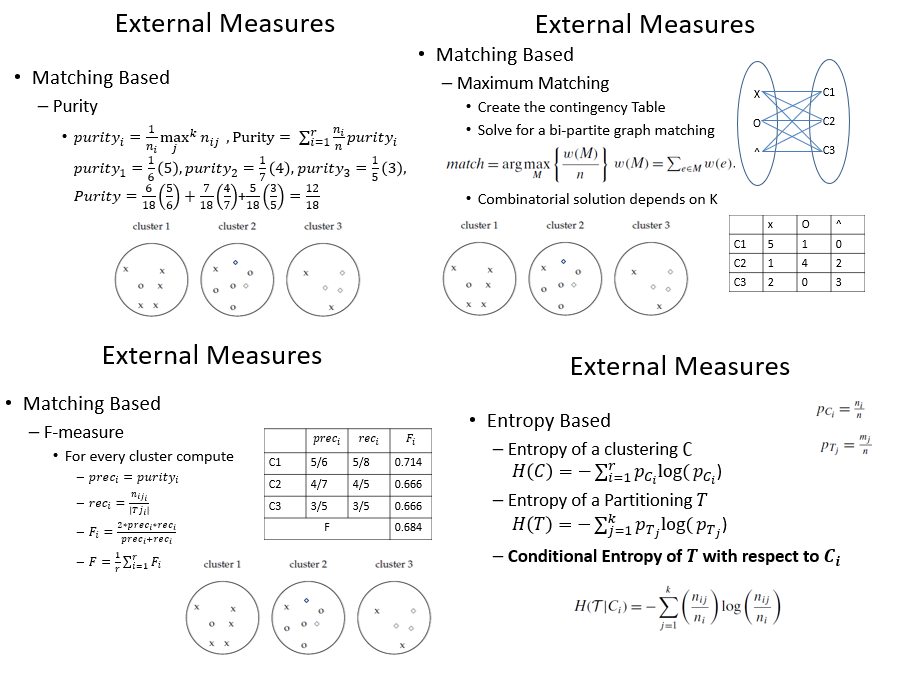
\includegraphics[width=1.5\textwidth]{Figures/externalmes.png}}
        \caption{\label{fig:figure11}External Measures}
    \end{figure}
    \item Conditional Entropy: measures how the clustering reduced the entropy of the ground truth,min value=0, max value = entropy of ground truth. The lower the value of this the better. For a perfect clustering, the conditional entropy value is zero, whereas the worst possible conditional entropy value is log k.
    \item For Jaccard and Rand indices, the larger the better. A prefect clustering has a value of 1 for both, Jaccard Index favors a clustering that puts points from the same ground truth partition together disregarding points not in the same ground truth partition appearing together.
    \begin{figure}[H]
        \centerline{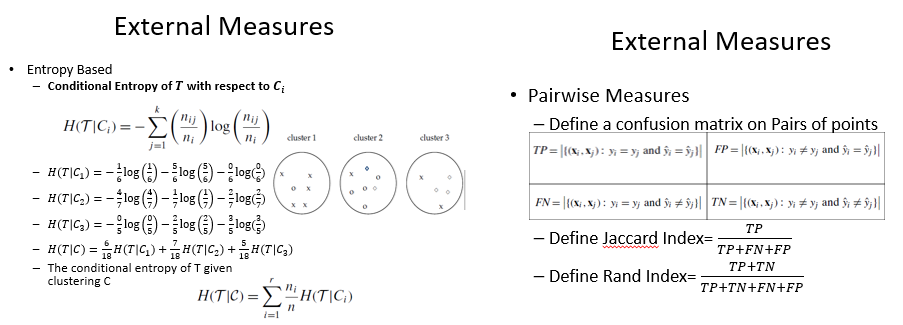
\includegraphics[width=1.5\textwidth]{Figures/externalmes2.png}}
        \caption{\label{fig:figure12}External Measures: Continue}
    \end{figure}
    \begin{figure}[H]
        \centerline{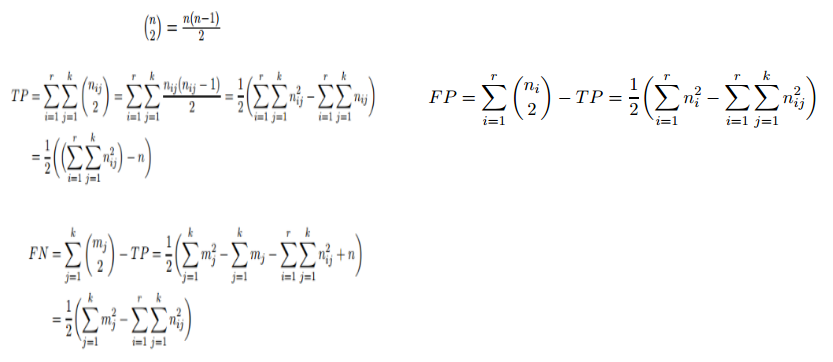
\includegraphics[width=1.5\textwidth]{Figures/externalmes3.png}}
        \caption{\label{fig:figure13}External Measures: Continue}
    \end{figure}
    $$TN = N- (TP + FP + FN)$$
    \[ purity(D_j) = \operatorname*{max}_i {\frac{n_{ij}}{n_j}}\] 
    \newpage
    \item Internal Measures treat with Clustering C as cut in a proximity (distance) matrix. The Graph(V,E) has V points and E edges. Edge weight is the proximity between two points. Given any subsets S,R (subset from V), define W(S,R) as the sum of the weights on all edges with one vertex in S and the other in R, given as
    \begin{figure}[H]
        \centerline{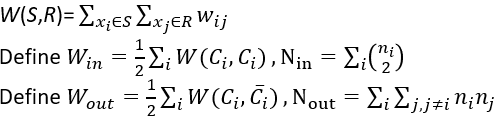
\includegraphics[width=0.8\textwidth]{Figures/internalmes.png}}
        \caption{\label{fig:figure14}Rules to get internal Measures}
    \end{figure}
    \begin{figure}[H]
        \centerline{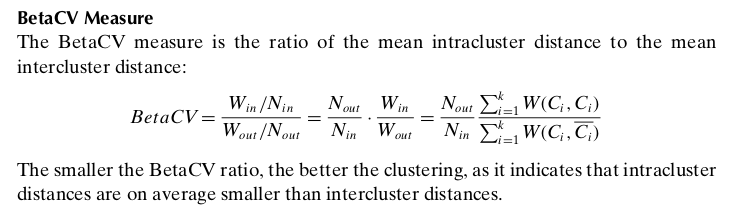
\includegraphics[width=1.1\textwidth]{Figures/beta.png}}
        \caption{\label{fig:figure15}Beta CV Measure}
    \end{figure}
    \begin{figure}[H]
        \centerline{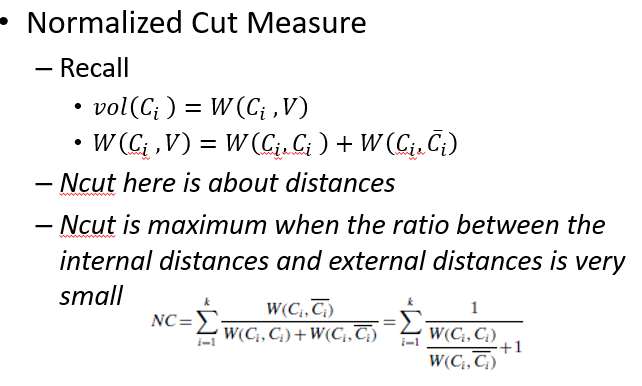
\includegraphics[width=0.9\textwidth]{Figures/internalmes2.png}}
        \caption{\label{fig:figure16}Normalized Cut measure}
    \end{figure}
    \begin{figure}[H]
        \caption{\label{fig:figure}Internal Measures Example}
        \centerline{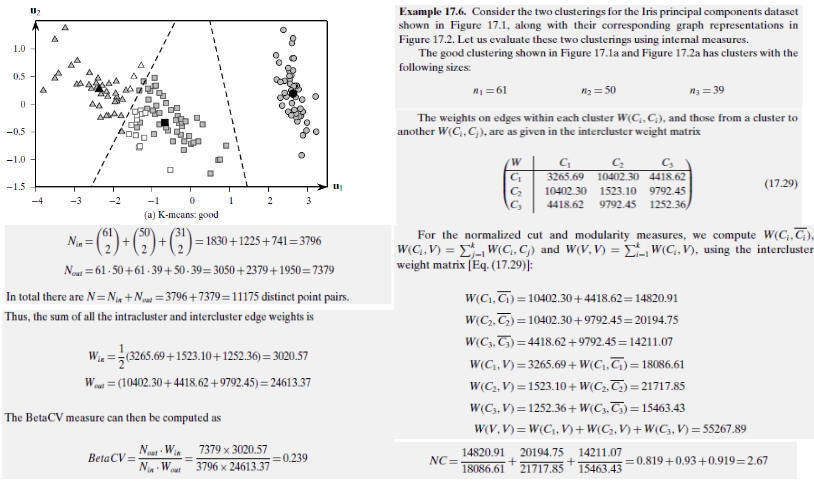
\includegraphics[width=1.5\textwidth]{Figures/cluster}}
    \end{figure}
    \item Beta-CV: The lower the better, measures the ratio internal cluster weights to cluster separation distance.This indicates that intracluster distances are on average smaller than intercluster distances.
    \item Normalized cut: The higher the value of this, the better it is, this is because we use a distance matrix and not a similarity matrix. The maximum possible value of NC is k.
\end{itemize}